%!TEX root = ../Electrodynamics.tex
\subsection{Общая постановка задачи о собственных электромагнитных колебаниях в полых резонаторах с идеально проводящими
стенками. Действительность собственных частот идеального резонатора.}

\begin{figure}[h!]
    \centering
    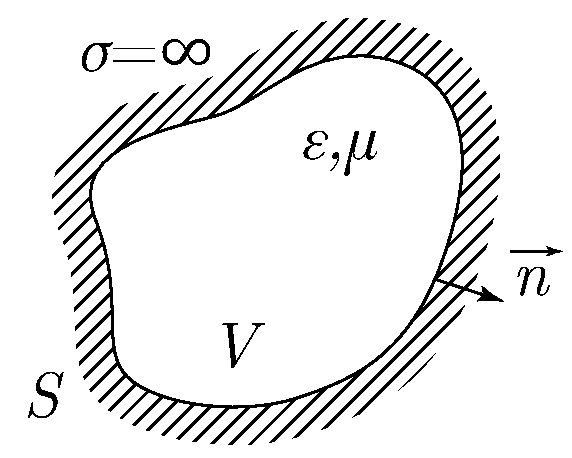
\includegraphics[width = .3\linewidth]{img/12-1.pdf}
    \caption{Резонатор произвольной формы}
\end{figure}
Рассматриваем любую металлическую полость произвольной формы. Для идеального проводника выполняются граничные условия на
поверхности проводника $S$:
\begin{equation}
    E_{\tau}\big|_S = 0,~ H_n\big|_S = 0    
\end{equation}
Для собственных колебаний необходимо решить систему из уравнений Максвелла:
\begin{equation}
    \left\{
    \begin{aligned}
        &\Rot{\vec{H}} = i\frac{w}{c}\epsilon \vec{E}\\
        &\Rot{\vec{E}} = -i\frac{w}{c}\mu \vec{H}
    \end{aligned}\right.    
\end{equation}
Возьмем ротор от второго уравнения, и подставим $\Rot{\vec{H}}$ из первого, получим:
\begin{equation}
    -\Rot{\Rot{\vec{E}}}+k^2\vec{E} = 0,~ k = \frac{w}{c}\sqrt{\mu\epsilon}    
\end{equation}
Нас интересует решение
\begin{equation}
    \Delta \vec{E} +k^2 \vec{E} = 0, \text{ при условии}
    \left\{
    \begin{aligned}
        &\Div{\vec{E}} = 0\\
        &E_{\tau}\big|_S = 0
    \end{aligned}\right.    
\end{equation}
$-\Rot{\Rot{\vec{A}}}$ представляется в виде:
\begin{equation}
    -\Rot{\Rot{\vec{A}}}  = \Delta \vec{A} -\grad \Div \vec{A} 
\end{equation}
В декартовой системе координат:
\begin{equation}
    \Delta E_{x,y,z} +k^2 E_{x,y,z} = 0
\end{equation}
Докажем свойства решения этой задачи.

\textbf{Спектр собственных частот действителен}

\begin{equation}
    \Div \left[\vec{E}\times \vec{H}^*\right]  = \vec{H}^*\Rot \vec{E} - \vec{E}\Rot\vec{H}^*   
\end{equation}
Подставим сюда выражения для ротора из уравнений Максвелла:
\begin{align*}
    \Div \left[\vec{E}\times \vec{H}^*\right]  =& \vec{H}^*(-\frac{iw}{c}\mu\vec{H})-\frac{1}{ik_0\epsilon}\Rot\vec{H} \Rot\vec{H}^* = \\
    & = -ik_0\mu |\vec{H}|^2-\frac{1}{ik_0\epsilon}|\Rot\vec{H}|^2
\end{align*}
Проинтегрируем по объему резонатора, пользуясь теоремой Остроградского-Гаусса:
\begin{align*}
    \int \limits_V \Div &\left[\vec{E}\times \vec{H}^*\right] \dd V  = \oiint \limits_S \left[\vec{E}\times \vec{H}^*\right]_n \dd S = 0,\text{ т.к.} E_\tau = 0 \Rightarrow \\
    &\Rightarrow  \int \limits_V-ik_0\mu |\vec{H}|^2-\frac{1}{ik_0\epsilon}|\Rot\vec{H}|^2 \dd V = 0
\end{align*}
Тогда
\begin{equation}
    k_0^2 =\frac{\int \limits_V\frac{1}{\epsilon}|\Rot\vec{H}|^2 \dd V}{\int \limits_V\mu|\vec{H}|^2 \dd V}   >0,\text{ при } \epsilon,\mu>0  
\end{equation}
т.е. спектр частот действителен. Частота моды $p$ $w_p$ - действительна при $\sigma = \infty,\epsilon,\mu>0$. Колебания происходят без
затухания:
\begin{equation}
    \underbrace{\int \limits_V \frac{\epsilon|\vec{E}|^2}{16\pi}\dd V }_{\overline{W^e}}=  \underbrace{\int \limits_V \frac{\mu|\vec{H}|^2}{16\pi}\dd V}_{\overline{W^m}}   
\end{equation}
Происходит перекачка энергии $\overline{W^e} \Leftrightarrow \overline{W^m}$. При пустом резонаторе $\epsilon = \mu =
1$:
\begin{equation}
    k_p = \frac{w_p^{(0)}}{c}    
\end{equation}
Если $\epsilon,\mu>0$:
\begin{equation}
    w_p = \frac{k_p c}{\sqrt{\epsilon\mu}} = \frac{w_p^{(0)}}{\sqrt{\epsilon\mu}}    
\end{equation}